\documentclass{ashoka-crypto}
\usepackage{enumitem}
\usepackage{mathtools, graphicx}
\usepackage{verbatim}
\usepackage{listingsutf8}
\usepackage[utf8x]{inputenc}
\usepackage[T1]{fontenc}

\lstdefinestyle{ciphertext}{
    breaklines=true,
    breakatwhitespace=false,
    columns=fullflexible,
    keepspaces=true,
    showstringspaces=false,
    basicstyle=\ttfamily\small,
    frame=single,
    captionpos=b
}

\newcommand\comb[2][^n]{\prescript{#1\mkern-0.5mu}{}C_{#2}}

\graphicspath{{./images/}}

\author{Aryan Nath} % Your name
\problem{2} % Problem set number

\collab{none}
% or give names, e.g., \collab{Alyssa P. Hacker and A. Student}

\begin{document}

\section*{Problem 1}
\begin{figure}[h]
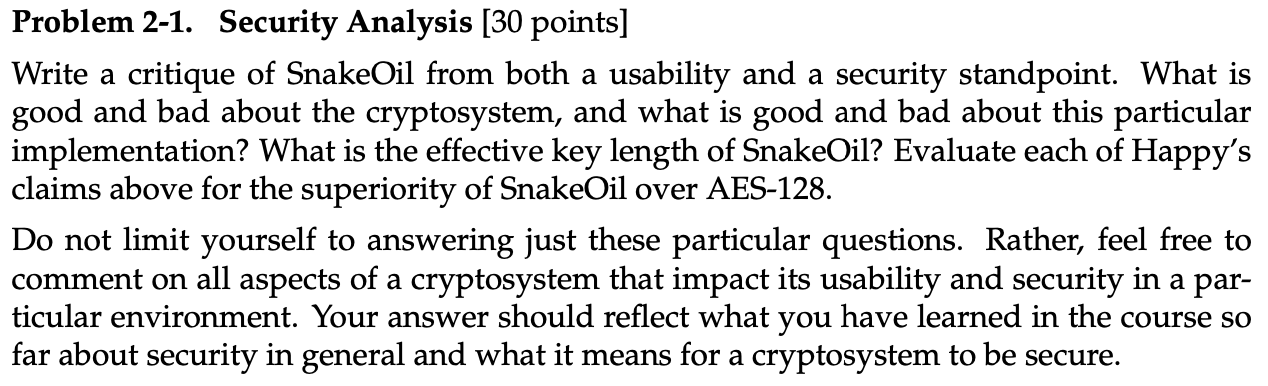
\includegraphics[width=17cm]{1}
\centering
\end{figure}
\begin{enumerate}[label=(\alph*)]
\item A good system is one which makes it very hard for an adversary to guess a message plaintext using just ciphertext and priors about the cryptosystem that have been published. There are more than one factors that need to be satisfied to make this problem hard for the adversary. Firstly, and most basically, the letters of the ciphertext should atleast be a shuffling of the plaintext - the adversary should not be able to just look at the ciphertext and guess the plaintext. The lesser information that the adversary is able to retrieve about the plaintext from just the ciphertext and the public parameters of the cryptosystem, the better is the cryptosystem, or more precisely, the probability of guessing the plaintext should be increased by having the ciphertext. A good cryptosystem will produce a ciphertext that will look completely random to the adversary, this should even be so for repeated letter plaintexts - which was not the case for the breakable cryptosystem from assignment 1. Besides randomness, the adversary should not be able to combine or perform operations on ciphertexts and get some meaningful information that they can use to break the cryptosystem. For example, if a cryptosystem decrypts the two messages 'Good morning, the weather is great today', and 'Good morning, I'm going for jog', now if the encryption is letter by letter, the adversary should not be able to for example subtract the ASCII values of the sets of letters and some representation of difference between the key values used to decrypt the two ciphertexts. Lastly, the cryptosystem should be resistant to brute force attacks. The adversary should not be able to efficiently check decryptions for all possible keys(brute force attack) in the key space and get the correct plaintext through some additional processing such as letter frequency analysis. A cryptosystem that does not satisfy any one of these factors is not a good cryptosystem and can be 'broken' by an adversary without knowing the encryption key. In case of usability, the encryption function should be computationally feasible otherwise the cryptosystem will be redundant.
\item Now let's consider the SnakeOil modification of AES-128/CBC. Firstly, if zeroes are interpreted as NUL/NULL, then this will not create a problem for decoding the texts where the ciphertext receiver can assume no NUL/NULL values in the text. For any other file type which can contain NUL/NULL values, there will be decoding errors as simply padding with 0's will not help the receiver identify the number of the 0's to remove as a 0 byte (NUL/NULL) can be a part of the plaintext. But just for the case of text files, this zero padding cryptosystem is good in the context of padding as the adversary cannot use the zero padding to perform operations on the ciphertext to retrieve information about the plaintext. The other modification made is the key management system. In terms of key generation, the XOR'ed master key will still be random because the XOR of two random values is also random. So just from this perspective as well, the cryptosystem is good as there are not a certain set of master keys that are more likely to occur in the key space that the adversary can use to guess the encryption key. Besides this, since Happy is still following AES for encryption, the randomness of the ciphertexts and inability to guess the plaintext with just the ciphertext will be preserved.
\item However, if the key shares are public, Happy has effectively reduced the key space size of AES-128 from $2^{128}$ to $\comb[100]{2}$. The adversary now has to just brute force check all possible pairs of key shares to generate a master key instead of trying for all possible $2^{128}$ encryption keys with undisclosed keys(making a subset of encryption keys public was already a big mistake). The key space is now fixed in terms of the public key shares and not 128 unkown bits per key. This made it \textit{feasible} for the adversary to brute force the effective key space and guess the plaintext after some processing like letter frequency analysis.
\item Beyond the three characteristics I have mentioned above, a cryptosystem is good if its ciphertexts are random, which can be measured using good confusion and diffusion values - how does a change in the jey and plaintext have in the ciphertext output, without either of the two being traceable from the ciphertext. Moreover, the security of the cryptosystem should rely completely on the key being kept secret so that the cryptosystem itself can be made public to other users for communication. Lastly, encryption and decryption with any key should be computationally feasible.
\end{enumerate}

\clearpage

\begin{figure}[h]
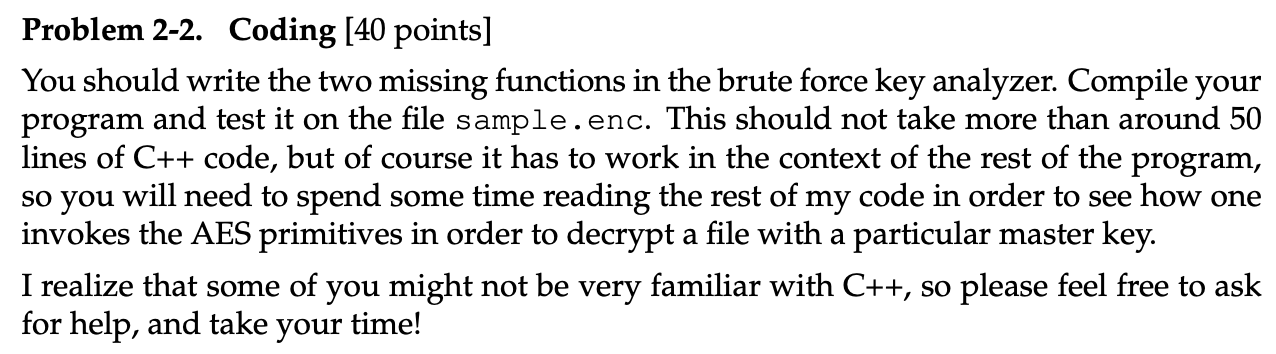
\includegraphics[width=17cm]{2}
\centering
\end{figure}

The code for this question has been submitted on google classroom.

The plaintext that I retrieved is:
\begin{verbatim}
This is a sample text that is encrypted using keyshares with key
indices 4 and 31.
\end{verbatim}

Files used:
\begin{itemize}
\item Frequency table: data/space.dat
\item keyshares hex codes: data/keyshares
\item file encrypted using snakeoil: data/sample.enc
\item output file: project\_root/output.txt
\end{itemize}

\clearpage

\begin{figure}[h]
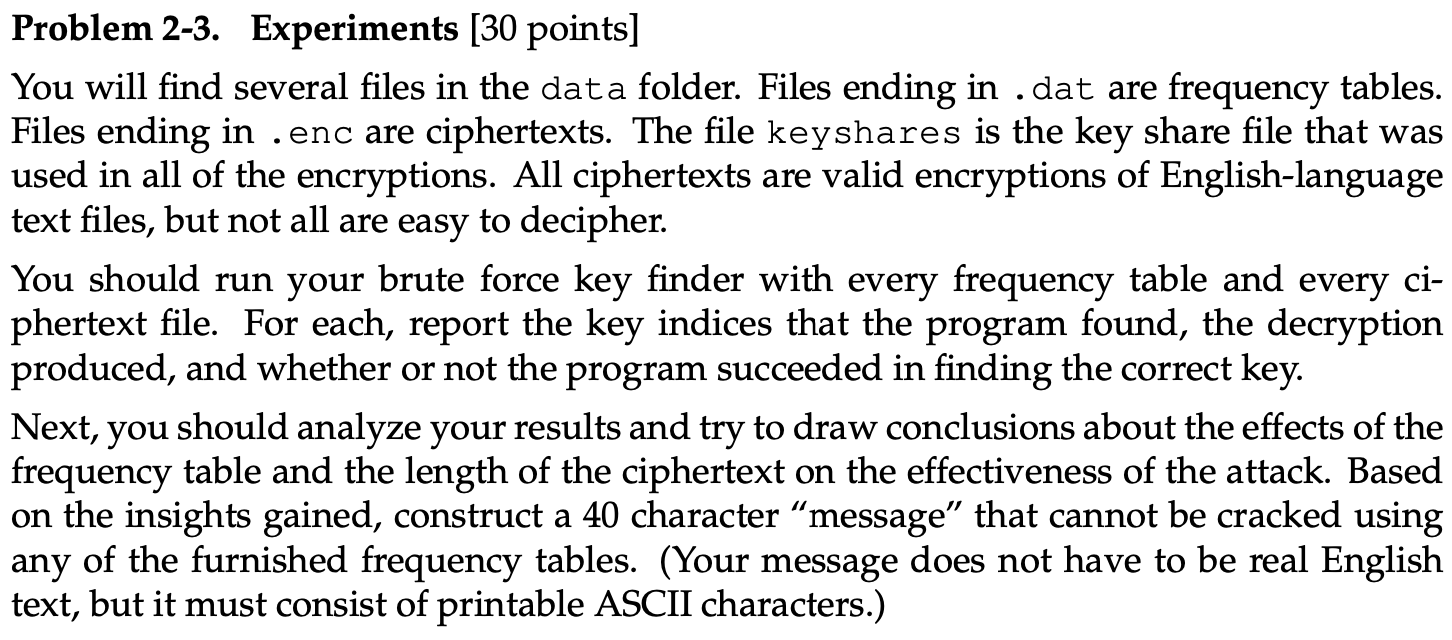
\includegraphics[width=17cm]{3}
\centering
\end{figure}

\begin{enumerate}
\item mystery1.enc

Length of ciphertext: 1488 bytes

\begin{enumerate}
\item frequency table used: merrywives.dat

Key Indices: 14 and 93
\begin{enumerate}
\item Decryption:

Four score and seven years ago our fathers brought forth on this continent, a new nation, conceived in Liberty, and dedicated to the proposition that all men are created equal. 

Now we are engaged in a great civil war, testing whether that nation, or any nation so conceived and so dedicated, can long endure. We are met on a great battle-field of that war. We have come to dedicate a portion of that field, as a final resting place for those who here gave their lives that that nation might live. It is altogether fitting and proper that we should do this. 

But, in a larger sense, we can not dedicate -- we can not consecrate -- we can not hallow -- this ground. The brave men, living and dead, who struggled here, have consecrated it, far above our poor power to add or detract. The world will little note, nor long remember what we say here, but it can never forget what they did here. It is for us the living, rather, to be dedicated here to the unfinished work which they who fought here have thus far so nobly advanced. It is rather for us to be here dedicated to the great task remaining before us -- that from these honored dead we take increased devotion to that cause for which they gave the last full measure of devotion -- that we here highly resolve that these dead shall not have died in vain -- that this nation, under God, shall have a new birth of freedom -- and that government of the people, by the people, for the people, shall not perish from the earth.

\item Success in decryption: Yes, the program was able to decrypt the ciphertext using the merriwives.dat frequency table.
\end{enumerate}
\item frequency table used: space.dat

Key Indices: 14 and 93
\begin{enumerate}
\item Decryption:

Four score and seven years ago our fathers brought forth on this continent, a new nation, conceived in Liberty, and dedicated to the proposition that all men are created equal. 

Now we are engaged in a great civil war, testing whether that nation, or any nation so conceived and so dedicated, can long endure. We are met on a great battle-field of that war. We have come to dedicate a portion of that field, as a final resting place for those who here gave their lives that that nation might live. It is altogether fitting and proper that we should do this. 

But, in a larger sense, we can not dedicate -- we can not consecrate -- we can not hallow -- this ground. The brave men, living and dead, who struggled here, have consecrated it, far above our poor power to add or detract. The world will little note, nor long remember what we say here, but it can never forget what they did here. It is for us the living, rather, to be dedicated here to the unfinished work which they who fought here have thus far so nobly advanced. It is rather for us to be here dedicated to the great task remaining before us -- that from these honored dead we take increased devotion to that cause for which they gave the last full measure of devotion -- that we here highly resolve that these dead shall not have died in vain -- that this nation, under God, shall have a new birth of freedom -- and that government of the people, by the people, for the people, shall not perish from the earth.

\item Success in decryption: Yes, the program was able to decrypt the ciphertext using the space.dat frequency table.
\end{enumerate}
\item frequency table used: ulysses.dat

Key Indices: 14 and 93
\begin{enumerate}
\item Decryption:

Four score and seven years ago our fathers brought forth on this continent, a new nation, conceived in Liberty, and dedicated to the proposition that all men are created equal. 

Now we are engaged in a great civil war, testing whether that nation, or any nation so conceived and so dedicated, can long endure. We are met on a great battle-field of that war. We have come to dedicate a portion of that field, as a final resting place for those who here gave their lives that that nation might live. It is altogether fitting and proper that we should do this. 

But, in a larger sense, we can not dedicate -- we can not consecrate -- we can not hallow -- this ground. The brave men, living and dead, who struggled here, have consecrated it, far above our poor power to add or detract. The world will little note, nor long remember what we say here, but it can never forget what they did here. It is for us the living, rather, to be dedicated here to the unfinished work which they who fought here have thus far so nobly advanced. It is rather for us to be here dedicated to the great task remaining before us -- that from these honored dead we take increased devotion to that cause for which they gave the last full measure of devotion -- that we here highly resolve that these dead shall not have died in vain -- that this nation, under God, shall have a new birth of freedom -- and that government of the people, by the people, for the people, shall not perish from the earth.

\item Success in decryption: Yes, the program was able to decrypt the ciphertext using the ulysses.dat frequency table.
\end{enumerate}
\item frequency table used: uniform.dat

Key Indices: 43 and 65
\begin{enumerate}
\item Decryption:
\begin{figure}[h]
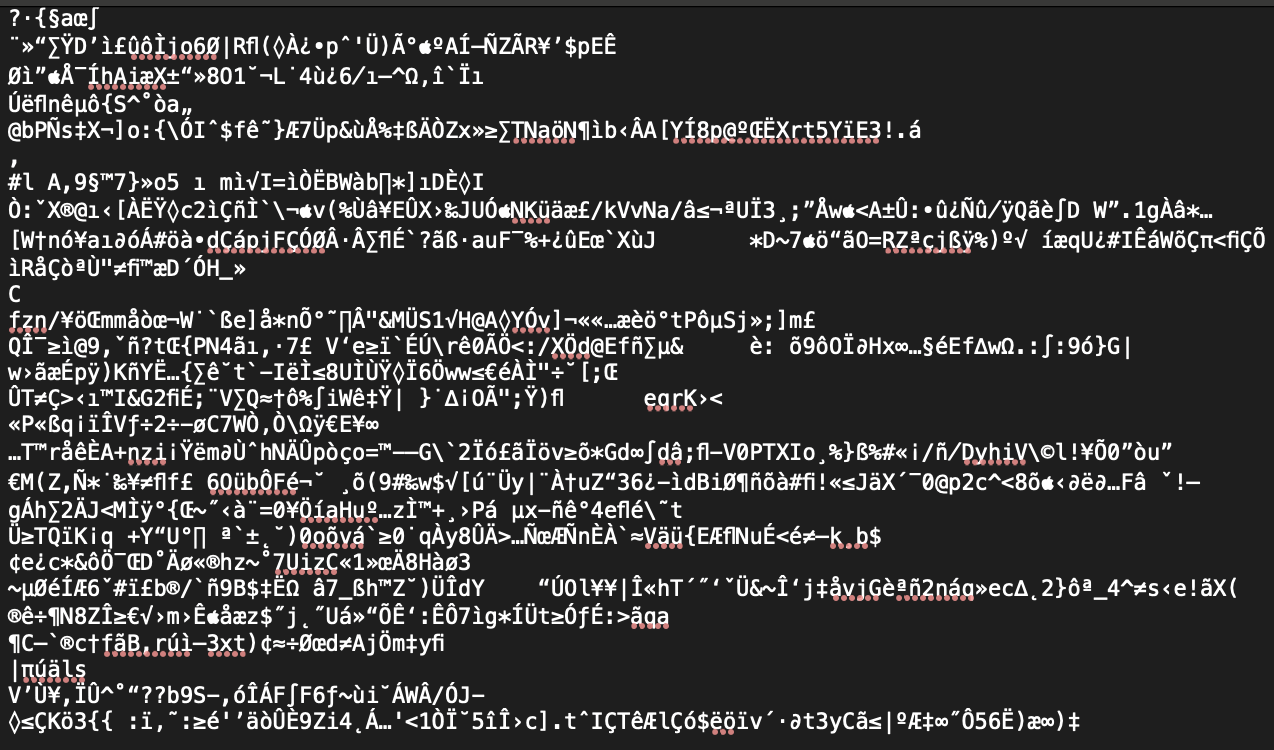
\includegraphics[width=12cm]{3_1_uniform}
\centering
\end{figure}

\item Success in decryption: No, the program was not able to decrypt the ciphertext using the uniform.dat frequency table.
\end{enumerate}
\end{enumerate}

\item mystery2.enc

Length of ciphertext: 736 bytes

\begin{enumerate}
\item frequency table used: merrywives.dat

Key Indices: 55 and 82
\begin{enumerate}
\item Decryption:

I have a dream that one day this nation will rise up and live out the true meaning of its creed: "We hold these truths to be self-evident: that all men are created equal." I have a dream that one day on the red hills of Georgia the sons of former slaves and the sons of former slaveowners will be able to sit down together at a table of brotherhood. I have a dream that one day even the state of Mississippi, a desert state, sweltering with the heat of injustice and oppression, will be transformed into an oasis of freedom and justice. I have a dream that my four children will one day live in a nation where they will not be judged by the color of their skin but by the content of their character. I have a dream today.

\item Success in decryption: Yes, the program was able to decrypt the ciphertext using the merriwives.dat frequency table.
\end{enumerate}
\item frequency table used: space.dat

Key Indices: 55 and 82
\begin{enumerate}
\item Decryption:

I have a dream that one day this nation will rise up and live out the true meaning of its creed: "We hold these truths to be self-evident: that all men are created equal." I have a dream that one day on the red hills of Georgia the sons of former slaves and the sons of former slaveowners will be able to sit down together at a table of brotherhood. I have a dream that one day even the state of Mississippi, a desert state, sweltering with the heat of injustice and oppression, will be transformed into an oasis of freedom and justice. I have a dream that my four children will one day live in a nation where they will not be judged by the color of their skin but by the content of their character. I have a dream today.

\item Success in decryption: Yes, the program was able to decrypt the ciphertext using the space.dat frequency table.
\end{enumerate}
\item frequency table used: ulysses.dat

Key Indices: 55 and 82
\begin{enumerate}
\item Decryption:

I have a dream that one day this nation will rise up and live out the true meaning of its creed: "We hold these truths to be self-evident: that all men are created equal." I have a dream that one day on the red hills of Georgia the sons of former slaves and the sons of former slaveowners will be able to sit down together at a table of brotherhood. I have a dream that one day even the state of Mississippi, a desert state, sweltering with the heat of injustice and oppression, will be transformed into an oasis of freedom and justice. I have a dream that my four children will one day live in a nation where they will not be judged by the color of their skin but by the content of their character. I have a dream today.

\item Success in decryption: Yes, the program was able to decrypt the ciphertext using the ulysses.dat frequency table.
\end{enumerate}
\item frequency table used: uniform.dat

Key Indices: 6 and 3
\begin{enumerate}
\item Decryption:
\begin{figure}[h]
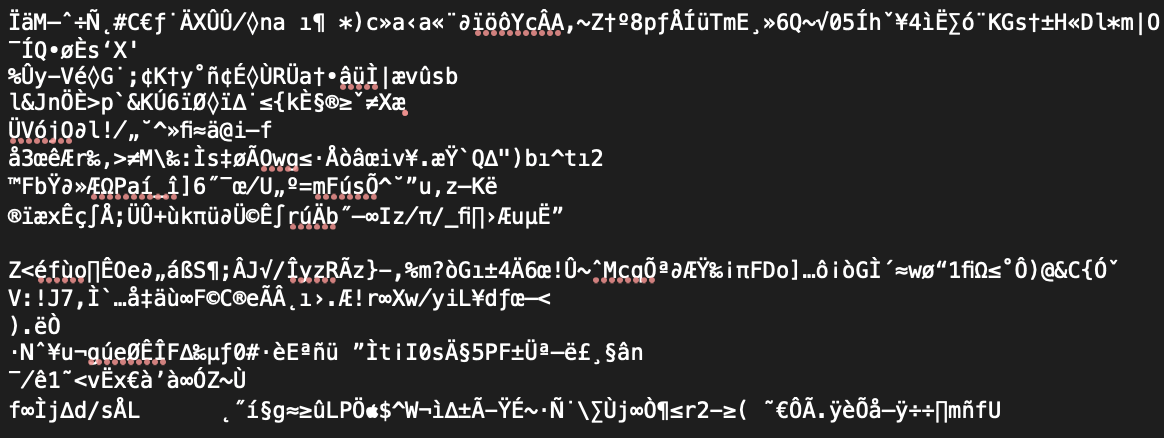
\includegraphics[width=12cm]{3_2_uniform}
\centering
\end{figure}

\item Success in decryption: No, the program was not able to decrypt the ciphertext using the uniform.dat frequency table.
\end{enumerate}
\end{enumerate}

\item mystery3.enc

Length of ciphertext: 64 bytes

\begin{enumerate}
\item frequency table used: merrywives.dat

Key Indices: 2 and 56
\begin{enumerate}
\item Decryption:

That's one small step for man; one giant leap for mankind.

\item Success in decryption: Yes, the program was able to decrypt the ciphertext using the merriwives.dat frequency table.
\end{enumerate}
\item frequency table used: space.dat

Key Indices: 2 and 56
\begin{enumerate}
\item Decryption:

That's one small step for man; one giant leap for mankind.

\item Success in decryption: Yes, the program was able to decrypt the ciphertext using the space.dat frequency table.
\end{enumerate}
\item frequency table used: ulysses.dat

Key Indices: 2 and 56
\begin{enumerate}
\item Decryption:

That's one small step for man; one giant leap for mankind.

\item Success in decryption: Yes, the program was able to decrypt the ciphertext using the ulysses.dat frequency table.
\end{enumerate}
\clearpage
\item frequency table used: uniform.dat

Key Indices: 3 and 18
\begin{enumerate}
\item Decryption:
\begin{figure}[h]
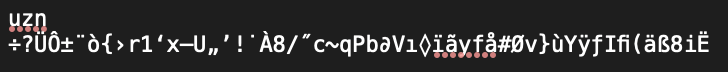
\includegraphics[width=8cm]{3_3_uniform}
\centering
\end{figure}

\item Success in decryption: No, the program was not able to decrypt the ciphertext using the uniform.dat frequency table.
\end{enumerate}
\end{enumerate}

\item mystery4.enc

Length of ciphertext: 16 bytes

\begin{enumerate}
\item frequency table used: merrywives.dat

Key Indices: 13 and 82
\begin{enumerate}
\item Decryption:

\begin{figure}[h]
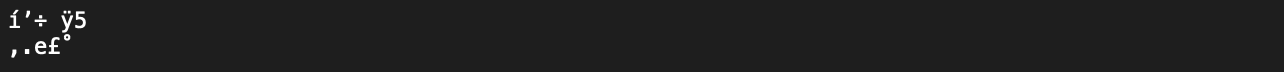
\includegraphics[width=12cm]{3_4_merrywives}
\centering
\end{figure}

\item Success in decryption: No, the program was not able to decrypt the ciphertext using the merriwives.dat frequency table.
\end{enumerate}
\item frequency table used: space.dat

Key Indices: 1 and 97
\begin{enumerate}
\item Decryption:

\begin{figure}[h]

\includegraphics[width=12cm]{3_4_space}
\centering
\end{figure}

\item Success in decryption: No, the program was not able to decrypt the ciphertext using the merriwives.dat frequency table.
\end{enumerate}
\item frequency table used: ulysses.dat

Key Indices: 13 and 82
\begin{enumerate}
\item Decryption:

\begin{figure}[h]
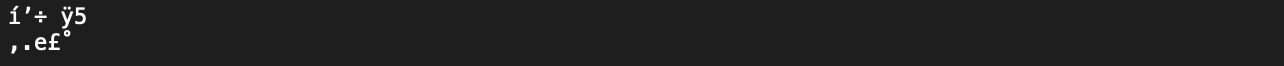
\includegraphics[width=12cm]{3_4_ulysses}
\centering
\end{figure}

\item Success in decryption: No, the program was not able to decrypt the ciphertext using the merriwives.dat frequency table.
\end{enumerate}
\clearpage 
\item frequency table used: uniform.dat

Key Indices: 0 and 1
\begin{enumerate}
\item Decryption:
\begin{figure}[h]
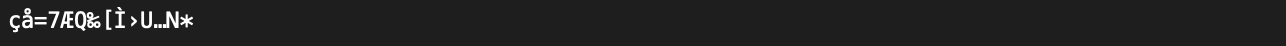
\includegraphics[width=12cm]{3_4_uniform}
\centering
\end{figure}

\item Success in decryption: No, the program was not able to decrypt the ciphertext using the uniform.dat frequency table.
\end{enumerate}
\end{enumerate}
\end{enumerate}

For the second part of the question, I need to find a plaintext such that after it has been encrypted with the selected keyshares pair, I wont be able to retrieve the correct plaintext using a frequency analysis attack without knowing the correct keyshares pair.

I noted that the \textit{uniform.dat} has assigned frequency of 1 to each of the ascii characters, and using it we cannot decrypt any of the given encrypted messages using a frequency analysis attack.

\textit{space.dat} assigns $0$ to all of the ascii characters except 1.

Let's first check if these two are able decrypt the ciphertext of a plaintext consisting of just a single letter.

I used $40$ $0$'s consecutively as my plaintext and I couldn't perform a successful bruteforce attack with any of the frequency tables.

Selected plaintext:
\begin{verbatim}
0000000000000000000000000000000000000000
\end{verbatim}

Key indices used for encryption: 4 and 62
\clearpage
\begin{enumerate}
\item merrywives.dat

Key Indices: 59 and 71

Decryption:

\begin{enumerate}
\item Decryption:
\begin{figure}[h]
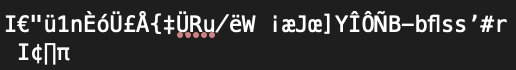
\includegraphics[width=10cm]{3_2_1_merrywives}
\centering
\end{figure}
\end{enumerate}
\item space.dat

Key Indices: 22 and 59

Decryption:

\begin{enumerate}
\item Decryption:
\begin{figure}[h]
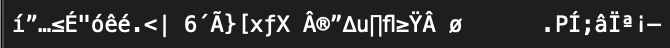
\includegraphics[width=12cm]{3_2_2_space}
\centering
\end{figure}
\end{enumerate}

\item space.dat

Key Indices: 59 and 71

Decryption:

\begin{enumerate}
\item Decryption:
\begin{figure}[h]
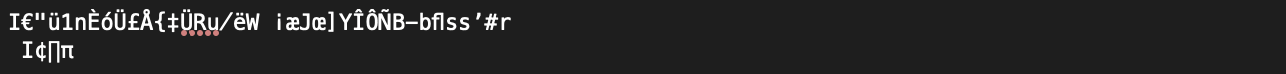
\includegraphics[width=12cm]{3_2_3_ulysses}
\centering
\end{figure}
\end{enumerate}

\item uniform.dat

Key Indices: 3 and 86

Decryption:

\begin{enumerate}
\item Decryption:
\begin{figure}[h]

\includegraphics[width=12cm]{3_2_4_uniform}
\centering
\end{figure}
\end{enumerate}
\end{enumerate}

Now let's analyze why I could not perform a successful frequency analysis attack using the frequency tables.

Firstly, I cannot directly infer that the reason for this was the ciphertext length since in the given encryptions, only \textit{mystery4.enc} had a small enough size - $16$ bytes - that one of reasons that none of the frequencies could be used to find the plaintext was because of the small size of the plaintext and hence the frequency distributions of the decryptions for not comparable to that expected from normal english sentences.

Secondly, I noticed that for none of the ciphertexts, the \textit{uniform.dat} frequency table could give a feasible distribution. The frequency table of uniform.dat is just 256 consecutive $1$'s. This means that based on \textit{unform.dat}, each ascii character is equally likely in the plaintext. So we were not able to use it to identify whether the frequency distribution of an obtained plaintext has a unique divergence with respect to uniform.dat. A similar case follows for \textit{space.dat}. In this frequency distribution, just a single ascii letter is expected to be present in the plaintext, and rest all of the ascii characters are expected to be absent. For the other two frequency tables, I considered having the frequency distribution of the plaintext as different as possible from the given frequency table. Having a plaintext consisting of the same character seems to work, even for \textit{space.dat} as long as the character is different from the which is assigned 1 in the frequency table. So any plaintext here consisting of all the same ascii character, other than the ascii character assigned 1 in the frequency table \textit{space.dat}, would work as the frequency distribution of such a plaintext would be quite different from all of the other frequency tables.

\end{document}

